\documentclass[aps,pra,reprint,amsmath,amssymb,longbibliography,floatfix]{revtex4-2}
\usepackage[T1]{fontenc}
\usepackage{graphicx}
\usepackage{booktabs}
\usepackage[colorlinks=true,linkcolor=blue,citecolor=blue,urlcolor=blue]{hyperref}
\newcommand{\ket}[1]{\lvert #1\rangle}
\newcommand{\bra}[1]{\langle #1\rvert}
\newcommand{\vac}{\ket{0000}}
\newcommand{\twist}{U_{\mathrm R}}
\newcommand{\Ptw}{P}
\newcommand{\Ftw}{F}

\begin{document}
\title{Replica twist entropy fails strong monotonicity under fermionic Gaussian measurements}
\author{Xiaojian Zeng}
\email{xiaojianzeng@foxmail.com}
\affiliation{PBC School of Finance, Tsinghua University, Beijing 100190, China}
\date{October 14, 2026}

\begin{abstract}
Replica twist entropy is a two-copy diagnostic of pure-state fermionic
non-Gaussianity with Gaussian invariance and product additivity.
We show that it does not satisfy strong monotonicity under recorded
fermionic Gaussian measurements. A coherent family with two occupation
flags has definite even parity and admits a closed replica overlap for
every integer number of four-mode resource blocks and every interior
rotation angle. Measuring one flag retains two pure branches of definite
parity. At the reflection-symmetric angle, an explicit 34-mode input
with outcome probabilities \(3/4\) and \(1/4\) increases the entropy on
average by exactly \(\ln(25836385/25165824)>0\).
For each fixed interior angle and nonzero branch probability, the input
entropy stays bounded while the mean output entropy grows linearly with
the number of blocks. This is an operational limitation of the finite-angle
replica diagnostic, without changing its established diagnostic properties.
The coherent-dilution mechanism is known in stabilizer resource theory;
the result here supplies its parity-preserving fermionic realization and
exact graded-copy calculation for the replica twist observable.
\end{abstract}
\maketitle

\section{Introduction}

Fermionic non-Gaussianity supplies resources beyond free-fermion dynamics.
Several ways to quantify it use covariance matrices, convolution, or
two-copy invariants \cite{LeoneBittelFermionic2026,Turkeshi2026,LyuBu2024,
Coffman2025,Tarabunga2026}. These constructions address different
operational questions. In particular, a faithful diagnostic that is
invariant under Gaussian unitaries and additive on products need not
decrease on average under Gaussian measurements.

Sun and Zhang introduced replica twist entropy as a finite-angle
two-copy probe of pure-state non-Gaussianity and applied it to
Sachdev--Ye--Kitaev dynamics \cite{SunZhang2026}.
Its finite-angle overlap probes correlations beyond the covariance
matrix. Their defining work establishes Gaussian invariance, additivity,
and diagnostic properties; it does not assert the strong-monotonicity
inequality examined here.

The distinction between logarithmic resource diagnostics and strong
monotones has a close precedent in stabilizer theory.
Haug and Piroli showed that stabilizer entropies fail strong
monotonicity using coherent dilution \cite{HaugPiroli2023}.
Leone and Bittel subsequently distinguished logarithmic stabilizer
monotones from their strongly monotone linear counterparts and gave
a flagged construction \cite{LeoneBittelMagic2024}.
We use this known idea in the fermionic setting. Two flags enforce
fermion-parity superselection, and the rotation amplitude must be
computed with anticommuting copies.
The contribution is an explicit family for the actual replica twist
functional, its closed all-angle expression, a rational finite-mode
counterexample, and unbounded average failure at every fixed interior
angle. The four-mode block used below is itself a qubit stabilizer
state, so the calculation is not an identification of stabilizer and
fermionic resource measures.

\section{Observable and operational question}
\label{sec:model}

Let \(\mathcal H_N\) be the Fock space of \(N\) complex fermionic modes.
Hermitian Majoranas \(\gamma_j\), \(j=1,\ldots,2N\), obey
\(\{\gamma_j,\gamma_k\}=2\delta_{jk}\).
All input vectors are normalized parity eigenstates,
\(\Pi_N\ket{\psi}=\epsilon\ket{\psi}\), with
\(\epsilon=\pm1\). Coherence between the two parity sectors is excluded.
On two graded copies, a register-first ordinary tensor representation is
\begin{equation}
 \gamma_j^{(1)}=\gamma_j\otimes I,\qquad
 \gamma_j^{(2)}=\Pi_N\otimes\gamma_j .
 \label{eq:graded}
\end{equation}
These Majoranas anticommute across copies as well as within each copy.
The replica rotation and its overlap are
\begin{align}
 \twist(\alpha)&=\exp\!\left[
   \frac{\alpha}{2}\sum_{j=1}^{2N}
       \gamma_j^{(1)}\gamma_j^{(2)}\right],\label{eq:UR}\\
 \Ftw_N(\psi;\alpha)&=\bra{\psi}^{\otimes2}
       \twist(\alpha)\ket{\psi}^{\otimes2},\label{eq:F}\\
 \Ptw_N(\psi;\alpha)&=-\ln \Ftw_N(\psi;\alpha),
       \qquad 0<\alpha<\frac{\pi}{2}.\label{eq:P}
\end{align}
Angles and entropies are dimensionless, and logarithms are natural.
The positive Majorana-string expansion recalled in Appendix~\ref{app:strings}
gives \(0<\Ftw_N\leq1\), so no logarithm-branch convention is needed.
The factor \(1/2\) in Eq.~\eqref{eq:UR} is part of the source convention;
replacing the graded second copy by \(I\otimes\gamma_j\) changes the model.

Pure Gaussian states have \(\Ptw=0\). Gaussian-unitary invariance
and additivity for fixed-parity product states are established
properties \cite{SunZhang2026}. A strong monotone would further obey
\begin{equation}
 \Ptw_N(\psi;\alpha)\ \geq\
       \sum_{a:p_a>0}p_a\Ptw_{N_a}(\phi_a;\alpha)
 \label{eq:strong}
\end{equation}
under Gaussian protocols with recorded pure outcomes.
Here the allowed primitives are even quadratic-Hamiltonian unitaries,
pure Gaussian ancillas of definite parity, occupation measurements,
and conditional Gaussian operations. A removed mode is refined into
a recorded occupation measurement; the compared output branches are pure.
No formula for a general mixed output is assumed.

It suffices to violate Eq.~\eqref{eq:strong} with one allowed occupation
measurement, retaining both outcomes. The original question fixes
\(\alpha=\pi/4\); the same family also permits an exact answer at
every fixed interior angle.

\section{A parity-preserving family and its overlap}
\label{sec:family}

Define the locally even four-mode vectors
\begin{equation}
 \ket V=\vac,\qquad
 \ket C=\frac{\ket{0000}+\ket{1111}}{\sqrt2}.
 \label{eq:VC}
\end{equation}
For an integer \(m\geq1\) and \(0<q<1\), set \(p=1-q\) and
\begin{align}
 \ket{A_m}&=\ket{00}\ket V^{\otimes m},&
 \ket{B_m}&=\ket{11}\ket C^{\otimes m},\label{eq:AB}\\
 \ket{\psi_{m,q}}&=\sqrt p\,\ket{A_m}
                  +\sqrt q\,\ket{B_m},&
 N&=4m+2.\label{eq:family}
\end{align}
The two flag modes precede the resource blocks in Fock order.
The flags make \(A_m\) and \(B_m\) orthogonal; every supported word
has even occupation. Thus the input is normalized and has definite
even total parity. Its preparation by free operations is not assumed.
The second flag ensures that the superposition respects parity
superselection.

Measuring the occupation of the first flag gives
\begin{align}
 (p_0,\ket{\phi_0})&=(p,\ket0\ket V^{\otimes m}),\nonumber\\
 (p_1,\ket{\phi_1})&=(q,\ket1\ket C^{\otimes m}).
 \label{eq:branches}
\end{align}
Both outcomes are recorded, both outputs are normalized pure states,
and their remaining parities are respectively even and odd.
There is no ancillary resource or additional gate in this operation.

\subsection{Graded rotation}

Write \(f_\ell^{(r)}
=(\gamma_{2\ell-1}^{(r)}+i\gamma_{2\ell}^{(r)})/2\).
Using the cross-copy CAR in Eq.~\eqref{eq:graded},
\begin{equation}
 \twist(\alpha)=\exp\!\left[\alpha\sum_{\ell=1}^N
 \left(f_\ell^{(1)\dagger}f_\ell^{(2)}
       -f_\ell^{(2)\dagger}f_\ell^{(1)}\right)\right].
 \label{eq:passive}
\end{equation}
It fixes the joint vacuum. With \(u=\cos\alpha\) and \(v=\sin\alpha\),
its action on creation operators is
\begin{align}
 \twist f_\ell^{(1)\dagger}\twist^\dagger
   &=u f_\ell^{(1)\dagger}-v f_\ell^{(2)\dagger},\nonumber\\
 \twist f_\ell^{(2)\dagger}\twist^\dagger
   &=v f_\ell^{(1)\dagger}+u f_\ell^{(2)\dagger}.
 \label{eq:creators}
\end{align}
The corresponding one-particle matrix is
\begin{equation}
 R=\begin{pmatrix}uI&vI\\-vI&uI\end{pmatrix}.
 \label{eq:R}
\end{equation}
For ordered occupied row and column lists \(J,K\), the Fock-space
matrix element is the occupied minor \(\det R[J,K]\).
This follows by antisymmetrically expanding the transformed creation
operators, and retains the fermionic ordering signs.

In particular, an ordered \(k\)-particle word in one copy and vacuum
in the other returns with amplitude \(u^k\).
Complete transfer has amplitude \(v^k\), or \((-v)^k\) in the reverse
direction. The \(k\) used below is even, so these transfer amplitudes
are positive. The summed occupation of each physical mode across
the two copies is conserved; different occupation words cannot
contribute to the same return or complete-transfer matrix element.

\subsection{Exact contraction}

For one resource block, the replicated vacuum and fully occupied
terms each return with amplitude one. The other two replicated terms
give return and transfer amplitudes \(u^4\) and \(v^4\).
Consequently,
\begin{align}
 f(\alpha):=\Ftw_4(C;\alpha)
   &=\frac12+\frac12(u^4+v^4)\nonumber\\
   &=1-\frac14\sin^2(2\alpha).
 \label{eq:f}
\end{align}
Thus \(3/4\leq f(\alpha)<1\) on the interior domain, and
\(f(\pi/4)=3/4\).

In the doubled state, \(A_mA_m\), \(B_mB_m\), and the span of
\(A_mB_m,B_mA_m\) have respectively zero, two, and one particles
across the first-flag copies. Conservation separates these sectors.
Their contributions are \(p^2\), \(q^2 f(\alpha)^m\), and a cross term.
Local factorization introduces no extra signs: in moving from
register-first to block-first Fock order, each crossing interchanges
two even local occupation words. Its sign is therefore \(+1\).

The total weight of components of \(B_m\) with \(r\) occupied
four-mode blocks is \(2^{-m}\binom mr\).
Each such occupation word has \(k=2+4r\) particles.
The return and complete-transfer contributions give
\begin{align}
 K_m(\alpha)
   &=2^{-m}\sum_{r=0}^m\binom mr
       \left(u^{2+4r}+v^{2+4r}\right)\nonumber\\
   &=u^2\left(\frac{1+u^4}{2}\right)^m
     +v^2\left(\frac{1+v^4}{2}\right)^m.
 \label{eq:K}
\end{align}
The full parent overlap is therefore
\begin{equation}
 \boxed{\Ftw_{4m+2}(\psi_{m,q};\alpha)
      =p^2+q^2 f(\alpha)^m+2pq K_m(\alpha).}
 \label{eq:parent}
\end{equation}
This is an exact finite-mode identity for all stated \(m,q,\alpha\),
with no omitted channels or large-system approximation.
The remaining number-state flag in each measured branch is Gaussian.
Its crossings with the even resource blocks also have positive sign,
including for the odd output \(\phi_1\). Hence
\begin{equation}
 \Ftw_{4m+1}(\phi_0;\alpha)=1,\qquad
 \Ftw_{4m+1}(\phi_1;\alpha)=f(\alpha)^m.
 \label{eq:branchF}
\end{equation}
Keeping the measured mode as its recorded Gaussian number state
would give the same entropy.

\section{Exact finite violation and amplification}
\label{sec:violation}

For the recorded measurement, define the average increase
\begin{align}
 \Delta_{m,q}(\alpha)
  &:=\sum_b p_b\Ptw_{4m+1}(\phi_b;\alpha)
           -\Ptw_{4m+2}(\psi_{m,q};\alpha)\nonumber\\
  &=\ln \Ftw_{4m+2}(\psi_{m,q};\alpha)
                -q m\ln f(\alpha).
 \label{eq:delta}
\end{align}
Strong monotonicity would require \(\Delta_{m,q}\leq0\).
At \(\alpha=\pi/4\), Eqs.~\eqref{eq:f} and \eqref{eq:K} simplify to
\begin{equation}
 f=\frac34,\qquad K_m=\left(\frac58\right)^m.
 \label{eq:midpoint}
\end{equation}
Choose \(m=8\), \(q=1/4\), and \(p=3/4\). The 34-mode input is
\begin{equation}
 \ket{\psi}=\frac{\sqrt3}{2}\ket{00}\vac^{\otimes8}
       +\frac12\ket{11}
          \left(\frac{\ket{0000}+\ket{1111}}{\sqrt2}\right)^{\otimes8}.
 \label{eq:witness}
\end{equation}
Its exact overlaps are
\begin{align}
 \Ftw_{\rm in}
   &=\frac9{16}+\frac1{16}\left(\frac34\right)^8
                      +\frac38\left(\frac58\right)^8\nonumber\\
   &=\frac{77509155}{134217728},\label{eq:Fin}\\
 (\Ftw_0,\Ftw_1)&=\left(1,\frac{6561}{65536}\right).
 \label{eq:Fout}
\end{align}
With both probabilities \(3/4,1/4\) included, the mean output
entropy is \(2\ln(4/3)\). Therefore
\begin{equation}
 \Delta_{8,1/4}(\pi/4)
       =\ln\!\left(\frac{25836385}{25165824}\right)>0.
 \label{eq:certificate}
\end{equation}
Strictness is the integer comparison
\(25836385>25165824>0\), rather than a floating-point test.
Integrating \(1/(1+x)\) gives the rational enclosure
\begin{equation}
 \frac{670561}{25836385}
 <\Delta_{8,1/4}(\pi/4)
 <\frac{670561}{25165824}.
 \label{eq:logbounds}
\end{equation}
The approximate value \(0.0262968862\) is only an illustration.
This one finite input and one allowed measurement disprove
the universal strong-monotonicity inequality at the specified angle.
No extension to more complicated protocols is needed.
The witness is not asserted to have the smallest possible mode count.

\begin{figure*}[t]
 \centering
 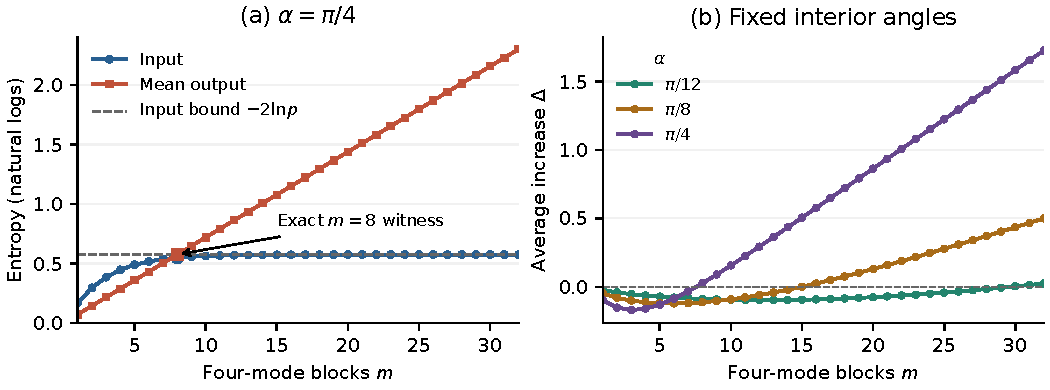
\includegraphics[width=0.96\textwidth]{figures/recorded_measurement.pdf}
 \caption{Recorded occupation measurement of the family
 in Eq.~\eqref{eq:family}, with \(q=1/4\).
 (a) At \(\alpha=\pi/4\), the input entropy stays below
 \(-2\ln(3/4)\), while the mean output entropy is
 \(m\ln(4/3)/4\).
 (b) The average increase from Eq.~\eqref{eq:delta} at three fixed
 interior angles. Markers denote integer \(m\); connecting lines
 guide the eye. Logarithms in the plot are evaluated in double
 precision. The \(m=8\) certificate is exact and does not rely on
 the plot. Plotting code was drafted with OpenAI Codex assistance;
 all values are generated from the displayed analytic expressions.}
 \label{fig:growth}
\end{figure*}

The same construction applies at every fixed
\(0<\alpha<\pi/2\) and \(0<q<1\).
Since \(K_m\geq0\), Eq.~\eqref{eq:parent} implies
\begin{align}
 \Ftw_{\rm in}&\geq p^2,&
 \Ptw_{\rm in}&\leq-2\ln p,\label{eq:bounded}\\
 \Delta_{m,q}(\alpha)&\geq
       q m[-\ln f(\alpha)]+2\ln p.
 \label{eq:linearbound}
\end{align}
The coefficient of \(m\) is strictly positive. In particular,
every integer satisfying
\begin{equation}
 m>\frac{-2\ln p}{q[-\ln f(\alpha)]}
 \label{eq:threshold}
\end{equation}
gives a strict finite counterexample.
For the parameters of Eq.~\eqref{eq:witness}, the right-hand side
equals eight. The additional positive terms in Eq.~\eqref{eq:Fin}
make the violation strict already at this equality.

For fixed interior \(\alpha\), each of
\((1+u^4)/2\), \((1+v^4)/2\), and \(f(\alpha)\) is less than one.
Consequently, as the finite integer \(m\) increases,
\begin{equation}
 \Ftw_{\rm in}\longrightarrow p^2,\qquad
 \Ptw_{\rm in}\longrightarrow-2\ln p,
 \label{eq:limit}
\end{equation}
while the mean output entropy is exactly
\(qm[-\ln f(\alpha)]\).
Thus the average increase is unbounded along this sequence
of finite-dimensional states, as illustrated in Fig.~\ref{fig:growth}.
No state in an infinite Fock space is assumed.

The sufficient threshold is not uniform near either angle endpoint:
\(f(\alpha)\to1\) as \(\alpha\to0\) or \(\pi/2\).
At the endpoints the family has unit overlap.
The growing-mode result therefore does not contradict a
fixed-mode small-angle covariance expansion or its associated
strong monotones \cite{SunZhang2026,LeoneBittelFermionic2026}.

\section{Verification and operational interpretation}
\label{sec:discussion}

The analytic contraction has two complementary representations.
Appendix~\ref{app:strings} derives the complete positive
Hermitian-Majorana expansion directly from the graded rotation.
Appendix~\ref{app:kernels} gives the exact local occupied-minor kernels.
Complete local Majorana-string sums reproduce these polynomial
identities and the rational certificate.
An independently programmed exterior-power calculation also
reproduces the same kernels and finite witness. Full graded
two-register calculations at \(N=6,10\) provide additional
floating-point checks of copy conventions and pure branches.
These checks do not replace the all-\(m\) factorization or establish
strictness through a tolerance. Exact arithmetic establishes
Eq.~\eqref{eq:certificate}.

OpenAI Codex language-model assistance was used in the state-family
search, derivations, code development, literature comparison,
and preparation of this draft. The native tool was OpenAI Codex CLI,
version 0.162.1. Recorded invocations requested model identifiers
\texttt{gpt-6.1-sol} with max reasoning and
\texttt{gpt-5.6-sol} with ultra reasoning; these identify local invocation
routing, rather than independently certified service weights.
Verification used explicit Majorana-string and occupied-minor computations,
including an independent computational reconstruction. Such computational checks
are distinct from human scientific review, which remains pending
for this local draft.

The limitation concerns using replica twist entropy to bound
average pure-state Gaussian conversion yield.
An occupation measurement reveals an extensive resource in one branch,
with both outcomes weighted by their actual probabilities.
Meanwhile the coherent parent retains a nonzero \(p^2\) contribution
to its two-copy overlap, bounding its logarithm.
This explains the failure without introducing a parity-coherent
input or discarding an unfavorable outcome.

Covariance-based strong monotones and Williamson-spectrum
majorization \cite{LeoneBittelFermionic2026,Turkeshi2026}
constrain different functionals.
The finite-angle replica quantity depends on higher-order
correlations \cite{SunZhang2026}. Likewise, sharing a graded
rotation with fermionic convolution does not identify a direct
overlap amplitude with the entropy of a reduced convolution
output \cite{LyuBu2024,Coffman2025}.
The bridge spectral framework is another established two-copy
representation; monotonicity of its spectral-support degree
is a different assertion from averaged monotonicity of a
logarithmic finite-angle amplitude \cite{Tarabunga2026}.

The coherent-dilution strategy is credited to its stabilizer
predecessors \cite{HaugPiroli2023,LeoneBittelMagic2024}.
The resource block \(C\) is a four-qubit stabilizer state, for example
with generators \(XXXX,ZZII,IZZI,IIZZ\), yet it has fermionic
overlap \(3/4\) at the symmetric angle. Thus the free theories
and the functions being tested are distinct. The substantive
fermionic calculation is the parity-legal family and its graded
all-angle overlap, rather than a new generic dilution mechanism.

The result leaves Gaussian invariance, product additivity,
faithfulness, and the source's SYK dynamical analysis intact.
It does not establish failure under deterministic pure-to-pure
conversion, a smallest counterexample, or an arbitrary mixed-state
extension. Its operational conclusion is that the given
finite-angle entropy fails Eq.~\eqref{eq:strong}, even for a
single recorded occupation measurement.

\begin{acknowledgments}
OpenAI Codex also assisted with manuscript drafting and preparation
of the reproducibility materials. Author review and confirmation
of the draft author details are pending.
\end{acknowledgments}

\section*{Data availability}
All central identities and the strict rational certificate are given
in the article. The accompanying local reproducibility materials contain
the exact Majorana-string checker, the independent occupied-minor
checker, the graded finite-mode replay, and the figure-generation
code with its data and software requirements.

\appendix
\section{Positive string expansion with the graded convention}
\label{app:strings}

Set \(A_j=\gamma_j^{(1)}\gamma_j^{(2)}\). Then
\(A_j^2=-I\), and \(A_jA_k=A_kA_j\) for \(j\ne k\).
With \(c=\cos(\alpha/2)\), \(s=\sin(\alpha/2)\),
\begin{equation}
 \twist(\alpha)=\prod_{j=1}^{2N}(cI+sA_j).
 \label{eq:prod}
\end{equation}
For an ordered subset \(S\) of length \(k\), let
\(\gamma_S=\prod_{j\in S}\gamma_j\) and \(h=k(k-1)/2\).
The ordinary register representation gives
\begin{equation}
 \prod_{j\in S}A_j=(-1)^h
                   \gamma_S\Pi_N^k\otimes\gamma_S.
 \label{eq:stringsign}
\end{equation}
Odd-\(k\) expectations vanish in a parity eigenstate.
For even \(k\), define the Hermitian string
\(\chi_S=i^h\gamma_S\). Its expectation is real, and the
expectation of Eq.~\eqref{eq:stringsign} in the replicated
input equals \(\lvert\bra\psi\chi_S\ket\psi\rvert^2\).
Expanding Eq.~\eqref{eq:prod} yields the published expression
\cite{SunZhang2026}
\begin{equation}
 \Ftw_N(\psi;\alpha)=
 \sum_{\substack{S\subseteq\{1,\ldots,2N\}\\ |S|\ {\rm even}}}
 c^{2N-|S|}s^{|S|}
       \lvert\bra\psi\chi_S\ket\psi\rvert^2 .
 \label{eq:strings}
\end{equation}
All weights are positive on the stated domain, and the identity
term is strictly positive. Unitarity supplies the upper bound one.
This derivation also specifies the string phase and the replica
angle independently of a tensor-copy commutation shortcut.

\section{Complete surviving local kernels}
\label{app:kernels}

For local vectors \(x_0,x_1\) define a replica kernel
\begin{equation}
 T_{abcd}=\bra{x_a}\bra{x_c}\twist(\alpha)
                   \ket{x_b}\ket{x_d}.
 \label{eq:T}
\end{equation}
Use \(x_0=\ket{00},x_1=\ket{11}\) for the flag kernel \(T^{\rm fl}\),
and \(x_0=V,x_1=C\) for the resource kernel \(T^{\rm res}\).
The occupied minors of Eq.~\eqref{eq:R} give
Table~\ref{tab:kernels}, where \(t=\sin^2\alpha\),
\(a=[1+(1-t)^2]/2\), and \(b=(1+t^2)/2\).
All ten omitted flag entries vanish: particle number in each
mode pair must match, so the flag occupations can only return
or transfer together. Resource entries paired with a zero
flag entry cannot contribute.

\begin{table}[b]
 \caption{The six surviving local replica kernels. Every value
 is an exact polynomial in \(t=\sin^2\alpha\).}
 \label{tab:kernels}
 \begin{ruledtabular}
 \begin{tabular}{ccc}
 \(abcd\)&\(T^{\rm fl}_{abcd}\)&\(T^{\rm res}_{abcd}\)\\
 \hline
 \(0000\)&\(1\)&\(1\)\\
 \(1111\)&\(1\)&\(1-t+t^2\)\\
 \(0011,\ 1100\)&\(1-t\)&\([1+(1-t)^2]/2\)\\
 \(0110,\ 1001\)&\(t\)&\((1+t^2)/2\)
 \end{tabular}
 \end{ruledtabular}
\end{table}

For example, the \(0011\) resource element averages the
vacuum return and the four-particle return, giving
\((1+u^4)/2\). The \(0110\) element averages the vacuum
and complete transfer, giving \((1+v^4)/2\).
The \(1111\) element is Eq.~\eqref{eq:f}.
The two-flag return and transfer are respectively \(u^2=1-t\)
and \(v^2=t\).

Writing \(z_0=\sqrt p\), \(z_1=\sqrt q\), contraction of the
four parent coefficients gives
\begin{align}
 \Ftw_{\rm in}
   &=\sum_{a,b,c,d=0}^1 z_a z_b z_c z_d
          T^{\rm fl}_{abcd}
          \bigl(T^{\rm res}_{abcd}\bigr)^m\nonumber\\
   &=p^2+q^2(1-t+t^2)^m
          +2pq\bigl[(1-t)a^m+t b^m\bigr].
 \label{eq:kernelcontract}
\end{align}
The block ordering signs are positive because every local
occupation word in both bra and ket has even parity.
This proves factorization for every integer \(m\), rather
than inferring it from finite tests.
Equation~\eqref{eq:kernelcontract} is exactly
Eq.~\eqref{eq:parent}.

\bibliography{references}
\end{document}
